\section{Ứng dụng ma trận trong vật lý và cơ học}\label{sec_1}

Muc tieu cua phan nay la su dung bieu dien ma tran de tim lai cac ket qua da trinh bay trong tuan truoc. Cac ket qua trinh bay duoi day hoan toan co the ap dung duoc cho cac he thong dao phuc tap co nhieu bac tu do hon. Ve mat toan hoc he dao dong 2 bac tu do voi cac he dao dong co 3,4,5 hoac tham chi 100 bac tu do la tuong tu.

\subsection{Làm quen với ma trận trong cơ học}
\subsubsection{Dao dong tu do}

De lam quen voi cac khai niem moi va on lai cac phep toan ma tran, chung ta se su dung lai vi du ve he thong dao dong 2 bac tu do da trinh bay trong tuan truoc \cref{fig_2dofs}.

\begin{figure}[htbp]
    \centering
    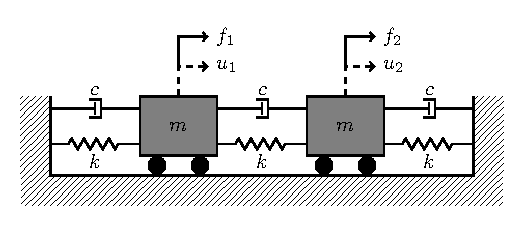
\includegraphics[width=1.\textwidth]{Tuan6/figure/mass_spring_damper_2dofs.pdf}
    \caption{2 dofs system}
    \label{fig_2dofs}
\end{figure}

Dieu dau tien trong khao sat mot he thong dao dong nhu tren hinh do la xac dinh cac modes dao dong rieng cua he. Cac modes dao dong rieng cua he la cac modes ma o do tat ca cac bac tu do bien thien theo thoi gian voi cung tan so. Vi day la mot he thong tuyen tinh nen nghiệm tổng quát (bất kỳ chuyển động nào của hai khối lượng) se được thể hiện dưới dạng tổ hợp tuyến tính của các nghiệm liên quan đến từng chế độ. De xac dinh cac modes dao dong rieng, ta bat dau voi viec khao xat he trong che do dao dong tu do. Co nghia la $c=0$ et $f_1=f_2=0$. Ta co phuong trinh can bang cho he ben tren.

\begin{equation}\label{eq_PT2dofs}
    \begin{cases}
        m \ddot{u}_1 + 2ku_1 - ku_2 = 0 \\
        m \ddot{u}_2 + 2ku_2 - ku_1 = 0 \\
    \end{cases}
\end{equation}

Bieu dien duoi dang ma tran.

\begin{equation}\label{eq_PTmatrix}
    \underbrace{\begin{bmatrix}
        m & 0\\ 0 & m
    \end{bmatrix}}_{\bf M}\underbrace{\begin{bmatrix}
        \ddot{u}_1 \\ \ddot{u}_2
    \end{bmatrix}}_{\ddot{\bf u}} +\underbrace{\begin{bmatrix}
        2k & -k \\ -k & 2k
    \end{bmatrix}}_{\bf K} \underbrace{\begin{bmatrix}
        u_1 \\ u_2
    \end{bmatrix}}_{\bf u} = \underbrace{\begin{bmatrix}
        0 \\ 0
    \end{bmatrix}}_{\bf O} 
\end{equation}

Cac bac tu do dao dong voi cung su phu thuoc theo thoi gian nen chung ta co:

\begin{equation}
    {\bf u} = \begin{bmatrix}
        u_1 \\ u_2
    \end{bmatrix} = {\bf X}cos(\Omega t)
\end{equation}

Thay vao PT phia tren, ta co:

\begin{equation}
    {\bf K}{\bf X} - \Omega^2{\bf M}{\bf X} = 0 \Leftrightarrow ({\bf K-\Omega^2{\bf M}}){\bf X} = 0
\end{equation}

Day la mot he phuong trinh tuyen tinh voi ve trai bang 0, co 2 truong hop xay ra do la he co 1 nghiem duy nhat ${\bf X} =0$ (vo nghia) va truong hop he co vo so nghiem (truong hop chung ta quan tam). Truong hop thu 2 xay ra khi va chi khi:

\begin{equation}
    det({\bf K}-\Omega^2{\bf M}) = 0
\end{equation}

Day la bai toan tim tri rieng cua ma tran. Giai he phuong trinh tren chung ta thu duoc:

\begin{equation}
    \Omega^2 =  \Omega_1^2 = \frac{k}{m} \quad \hbox{va} \quad \Omega^2 = \Omega_2^2 = \frac{3k}{m}
\end{equation}

Vector rieng cua he la:

\begin{equation}
    {\bf X} = {\bf X}_1 = \begin{bmatrix}
        1 \\ 1
    \end{bmatrix} \quad \hbox{va} \quad {\bf X} = {\bf X}_2 = \begin{bmatrix}
        1 \\ -1
    \end{bmatrix}
\end{equation}

Nghiem tong quat cua he la mot to hop tuyen tinh cua 2 modes nay. Vi vay ta co:

\begin{equation}
    {\bf u}=\underbrace{\left(A_1 \cos \left(\Omega_1 t\right)+B_1 \sin \left(\Omega_1 t\right)\right) {\bf X}_1}_{\hbox{Mode 1}}+\underbrace{\left(A_2 \cos \left(\Omega_2 t\right)+B_2 \sin \left(\Omega_2 t\right)\right) {\bf X}_2}_{\hbox{Mode 2}}
\end{equation}

Cac hang so $A_1, B_1, A_2, B_2$ duoc xac dinh bang cac dieu kien ban dau cua he.

\subsubsection{Dao dong cuong buc - Khong giam chan}

Xet truong hop $f_1 = F_1cos(\omega t)$ va $f_2 = F_2cos(\omega t)$. Dat ${\bf f} = \begin{bmatrix} F_1 \\ F_2\end{bmatrix}cos(\omega t) = {\bf F}cos(\omega t)$. Nghiem cua phuong trinh luc nay co dang ${\bf u} = \begin{bmatrix} U_1 \\ U_2\end{bmatrix}cos(\omega t) = {\bf U}cos(\omega t)$. Thay vao PT \cref{eq_PTmatrix}, ta co:

\begin{equation}
    -\omega^2{\bf M}{\bf U} + {\bf K}{\bf U} = {\bf F} \Rightarrow {\bf U} = (-\omega^2{\bf M}+{\bf K})^{-1} {\bf F}
\end{equation}

Ta tim duoc gia tri cua $U_1$ va $U_2$

\begin{equation}
    U_1 = \frac{F_1(2k-m\omega^2)+F_2k}{(k-m\omega^2)(3k-m\omega^2)} \quad \hbox{va} \quad U_2 = \frac{F_1k+F_2(2k-m\omega^2)}{(k-m\omega^2)(3k-m\omega^2)}
\end{equation}

\subsubsection{Dao dong cuong buc - co giam chan}

Truong hop he so $c \neq 0$, phuong trinh can bang duoc viet nhu sau:

\begin{equation}\label{eq_PT2dofs_c}
    \begin{cases}
        m \ddot{u}_1 + 2c\dot{u}_1 - c\dot{u}_2 + 2ku_1 - ku_2 = f1 \\
        m \ddot{u}_2 + 2c\dot{u}_2 - c\dot{u}_1 + 2ku_2 - ku_1 = f2 \\
    \end{cases}
\end{equation}

Dang ma tran cua phuong trinh nay la:

\begin{equation}\label{eq_PT2dofs_c_matrix}
    \underbrace{\begin{bmatrix}
        m & 0\\ 0 & m
    \end{bmatrix}}_{\bf M}\underbrace{\begin{bmatrix}
        \ddot{u}_1 \\ \ddot{u}_2
    \end{bmatrix}}_{\ddot{\bf u}} + \underbrace{\begin{bmatrix}
        2c & -c \\ -c & 2c
    \end{bmatrix}}_{\bf C}\underbrace{\begin{bmatrix}
        \dot{u}_1 \\ \dot{u}_2
    \end{bmatrix}}_{\dot{\bf u}} +\underbrace{\begin{bmatrix}
        2k & -k \\ -k & 2k
    \end{bmatrix}}_{\bf K} \underbrace{\begin{bmatrix}
        u_1 \\ u_2
    \end{bmatrix}}_{\bf u} = \underbrace{\begin{bmatrix}
        f_1 \\ f_2
    \end{bmatrix}}_{\bf f} 
\end{equation}

De giai phuong trinh nay, cach don gian nhat la chuyen ve dang so phuc. Vector ngoai luc $\bf f$ luc nay se duoc bieu dien o dang phuc ${\bf f} = {\bf F}e^{j\omega t}$. Nghiem cua phuong trinh se co dang ${\bf u} = {\bf U}e^{j\omega t}$.

Thay vao phuong trinh ta til duoc:

\begin{equation}\label{eq_nghiemphuc}
    \begin{aligned}
        {U}_1 &=\frac{\left(2 F_1+F_2\right) k-F_1 m \omega^2+j c\left(2 F_1+F_2\right) \omega}{\left(j c \omega+k-m \omega^2\right)\left(3 j c \omega+3 k-m \omega^2\right)}\\
        {U}_2 &=\frac{\left(F_1+2 F_2\right) k-F_2 m \omega^2+j c\left(F_1+2 F_2\right) \omega}{\left(j c \omega+k-m \omega^2\right)\left(3 j c \omega+3 k-m \omega^2\right)}
    \end{aligned}
\end{equation}

\textbf{\textcolor{red}{Cau hoi: se the nao neu vector ngoai luc ${\bf f}$ co dang ${\bf f} = {\bf F}_1cos(\omega_1t) + {\bf F}_2sin(\omega_2t)$ ?}}

